\documentclass[12pt]{article}

\usepackage[utf8]{inputenc}
\usepackage{latexsym,amsfonts,amssymb,amsthm,amsmath, graphicx, float, hyperref, caption}

\setlength{\parindent}{0in}
\setlength{\oddsidemargin}{0in}
\setlength{\textwidth}{6.5in}
\setlength{\textheight}{8.8in}
\setlength{\topmargin}{-0.5in}
\setlength{\headheight}{18pt}


\title{Assignment 1 — Applied Algorithms, T. II/2024–25}
\author{Austin Jetrin Maddison 6481268}

\begin{document}
	% \small
	
	\maketitle
	
	\vspace{0.5in}
	
	\subsection*{Problem 1. Las Vegas and Monte Carlo}
	
	
	a.i) We want to show the probablity of running time of Monte Carlo is atleast the worst running time which is $4f(n)$. We can use markov inqualities to bound it..
	\\

	\begin{align*}
		\textbf{P}(X \le \lambda ) & \le \frac{ E [ X ] }{ \lambda }\\
	\end{align*}

	\begin{align*}
		\textbf{P}(T(n) \le 4f(n) ) & \le \frac{f(n)}{4f(n)}\\
								    & \le \frac{1}{4}		
	\end{align*}
	
	a.ii) The worse-case running time happens at most 1/4 which produces incorrect answers. We can get the complement of the last answer...    

	\begin{align*}
		1 - \textbf{P}(T(n) \le 4f(n) ) &  \le 1 - \frac{1}{4} = \frac{3}{4}
	\end{align*}
	
	b.i) The LV algorithm running time is described as the follwing. Each iteration requires running A to produce an answer then run C to check the answer. So the running time for each trial is...
	
	\begin{align*}
		\text{1 iteration running time of LV} = f(n) + g(n)
	\end{align*}

	So the question is what is the expected iterations needed to run LV to get a correct answer. If p is the probablity of success then the expected $1/p$.

	\begin{align*}
		\text{Running time of LV} = \frac{1}{p}(f(n) + g(n))
	\end{align*}

	\vspace{2in} %Leave space for comments!
	
	
	\subsection*{Problem 2. Chernoff-Hoeffding With Bounds}
	2.1)
	\begin{align*}
		\mathrm{Pr}[X &> (1+\beta)\mu]\leq\exp\left(-\frac{\beta^{2}}{2+\beta}\mu H\right) \\
		\mathrm{Pr}[X &> (1+\varepsilon)\mu H]\leq\exp\left(-\frac{\varepsilon^{2}}{2+\varepsilon}\mu H\right)
	\end{align*}

	\begin{align*}
		(1 + \epsilon) \mu_{H} &= (1 + \beta) \mu \\
		\frac{\mu_{H}}{\mu} &= \frac{1 + \epsilon}{1 + \beta}\\
		% \beta $= \frac{\mu_{H}(1 + \epsilon)}{\mu}\\
	\end{align*}


	2.2)
	\begin{align*}
		\mathrm{Pr}[X &> (1+\beta)\mu]\leq\exp\left(-\frac{\beta^{2}}{2+\beta}\mu H\right) \\
		\mathrm{Pr}[X &> (1+\varepsilon)\mu H]\leq\exp\left(-\frac{\varepsilon^{2}}{2+\varepsilon}\mu H\right)
	\end{align*}

	\begin{align*}
		(1 + \epsilon) \mu_{H} &= (1 + \beta) \mu \\
		\frac{\mu_{H}}{\mu} &= \frac{1 + \epsilon}{1 + \beta}\\
		% \beta $= \frac{\mu_{H}(1 + \epsilon)}{\mu}\\
	\end{align*}

	2.3)
	\begin{align*}
		\mathrm{Pr}[X &> (1+\beta)\mu]\leq\exp\left(-\frac{\beta^{2}}{2+\beta}\mu H\right) \\
		\mathrm{Pr}[X &> (1+\varepsilon)\mu H]\leq\exp\left(-\frac{\varepsilon^{2}}{2+\varepsilon}\mu H\right)
	\end{align*}

	\begin{align*}
		(1 + \epsilon) \mu_{H} &= (1 + \beta) \mu \\
		\frac{\mu_{H}}{\mu} &= \frac{1 + \epsilon}{1 + \beta}\\
		% \beta $= \frac{\mu_{H}(1 + \epsilon)}{\mu}\\
	\end{align*}
	
	2.4)
	\begin{align*}
		\mathrm{Pr}[X &> (1+\beta)\mu]\leq\exp\left(-\frac{\beta^{2}}{2+\beta}\mu H\right) \\
		\mathrm{Pr}[X &> (1+\varepsilon)\mu H]\leq\exp\left(-\frac{\varepsilon^{2}}{2+\varepsilon}\mu H\right)
	\end{align*}

	\begin{align*}
		(1 + \epsilon) \mu_{H} &= (1 + \beta) \mu \\
		\frac{\mu_{H}}{\mu} &= \frac{1 + \epsilon}{1 + \beta}\\
		% \beta $= \frac{\mu_{H}(1 + \epsilon)}{\mu}\\
	\end{align*}
	\vspace{2in} %Leave space for comments!
	
	
	\subsection*{Problem 3. Rescaling Trick}
	(Statement of problem goes here.)\\
	
	\begin{proof}
		(Type your proof here.)
	\end{proof}
	
	\vspace{2in} %Leave space for comments!
	
	
	
	\subsection*{Problem 4. $x^2$ With $\pi$ Degrees of Freedom}
	(Statement of problem goes here.)\\
	
	\begin{proof}
		(Type your proof here.)
	\end{proof}
	
	\vspace{2in} %Leave space for comments!
	
	
	\subsection*{Problem 5. Simple Samplers.}
	(Statement of problem goes here.)\\
	
	\begin{proof}
		(Type your proof here.)
	\end{proof}
	
	\vspace{2in} %Leave space for comments!
	
	
	\subsection*{Problem 6. Median of Means}
	(Statement of problem goes here.)\\
	
	\begin{proof}
		(Type your proof here.)
	\end{proof}
	
	\vspace{2in} %Leave space for comments!
	
	
	\subsection*{Problem 7. Skip List}
	\vspace{20pt}
	\subsubsection*{Experimental Setup}
	Conducted our benchmarks using Google Benchmark~\cite{google-bench} on a system with the following hardware specifications:

\begin{itemize}
    \item \textbf{Processor}: 11th Gen Intel(R) Core(TM) i7-11370H 4C/8T CPU @ 3.3 GHz
    \item \textbf{Cache Hierarchy}:
    \begin{itemize}
        \item L1 Data: 48 KiB per core (\(\times 4\))
        \item L1 Instruction: 32 KiB per core (\(\times 4\))
        \item L2 Unified: 1280 KiB per core (\(\times 4\))
        \item L3 Unified: 12,288 KiB (shared)
    \end{itemize}
\end{itemize}

All benchmarks were compiled using \texttt{-Ox} optimization level with \texttt{MSVC} (version 19.42.34436) and executed in a single-threaded environment to minimize external interference. Memory usage was measured using the Windows API \texttt{GetProcessMemory()}~\cite{getprocessmemoryinfo}.\\

\subsubsection*{Questions And Experiments}
	
Q1.) Can we perform count coin tosses differently and is the alternative better?

\begin{figure}[H]
	\centering
	\begin{minipage}{0.32\textwidth}
		\centering
		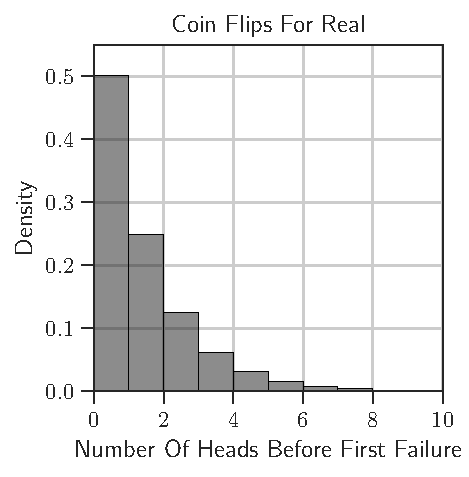
\includegraphics[width=\linewidth]{../notebook/plot/coin_flips_for_real.pdf}
		\label{fig:coin_flips_for_real}
	\end{minipage}\hfill
	\begin{minipage}{0.32\textwidth}
		\centering
		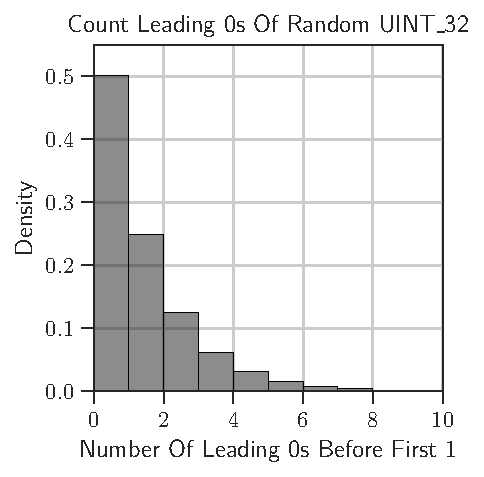
\includegraphics[width=\linewidth]{../notebook/plot/count_leading_0s_of_random_uint_32.pdf}
		\label{fig:coin_flips_count_leading}
	\end{minipage}\hfill
	\begin{minipage}{0.32\textwidth}
		\centering
		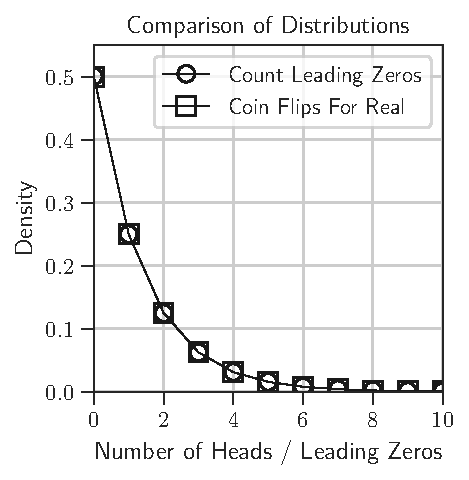
\includegraphics[width=\linewidth]{../notebook/plot/comparison_of_distributions.pdf}
		\label{fig:coin_flips_comparison}
	\end{minipage}
\end{figure}


\begin{table}[h]
	\centering
	\small
	\begin{tabular}{lrrr}
		\hline
		\textbf{Benchmark} & \textbf{Time (ns)} & \textbf{CPU (ns)} & \textbf{Iterations} \\
		\hline
		Coin Flip For Real & 29.8 & 29.3 & 22,400,000 \\
		\hline
		Coin Flip Count Leading 0s & 5.11 & 4.87 & 144,516,129 \\
	\end{tabular}
	\caption{Benchmark results comparing different coin flip implementations.}
	\label{tab:benchmark_results}
\end{table}

Q2.) How does varying max height change performance?

Q3.) Linked lists are known to be cache unfriendly, is there a way we can modify 

Q4.) How does it perform against a reputable ordered map?
\\\\
	
b.) Search algorithm of Skip List when start is at the bottom left corner in $O(\log(d))$ where d is the number of elements smaller than the key?
	

	
	\vspace{2in} %Leave space for comments!
	
	
	
	\subsection*{Problem 8. ($a,b$) tree. ($2, 3$) tree.}

	a.)	
	\begin{figure}[H] 
		\centering
		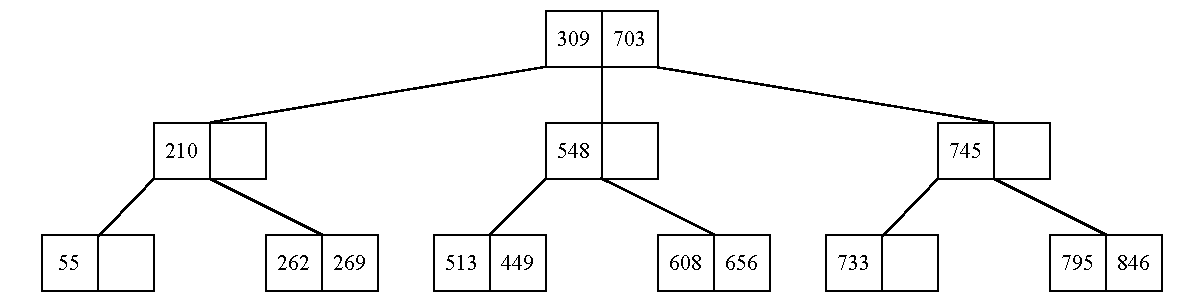
\includegraphics[width=0.9\linewidth]{Q8_a.drawio}
		\caption{Keys $733, 703, 608, 846, 309, 269, 55, 745, 548, 449, 513, 210, 795, 656, 262$ inserted into a $(2, 3)$ tree.}
		\label{fig:q8a}
	\end{figure}
	

	
	b.) 
	\begin{figure}[H] 
		\centering
		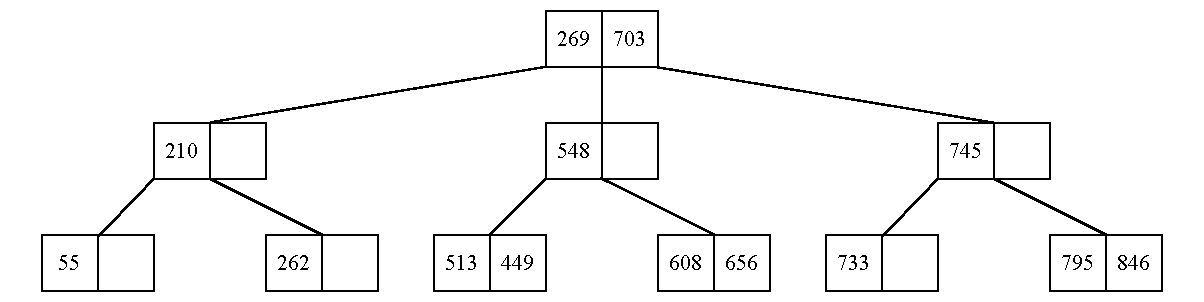
\includegraphics[width=0.9\linewidth]{Q8_b.drawio}
		\caption{Key 309 removed from Figure~\ref{fig:q8a} tree.}
		\label{fig:q8b}
	\end{figure}
	
	
\vspace{2in} %Leave space for comments!


\subsection*{Problem 9. B-Tree Speed}

\subsubsection*{Experimental Setup}
Conducted our benchmarks using Google Benchmark~\cite{google-bench} on a system with the following hardware specifications:

\begin{itemize}
	\item \textbf{Processor}: 11th Gen Intel(R) Core(TM) i7-11370H 4C/8T CPU @ 3.3 GHz
	\item \textbf{Cache Hierarchy}:
	\begin{itemize}
		\item L1 Data: 48 KiB per core (\(\times 4\))
		\item L1 Instruction: 32 KiB per core (\(\times 4\))
		\item L2 Unified: 1280 KiB per core (\(\times 4\))
		\item L3 Unified: 12,288 KiB (shared)
	\end{itemize}
\end{itemize}

All benchmarks were compiled using \texttt{-Ox} optimization level with \texttt{MSVC} (version 19.42.34436) and executed in a single-threaded environment to minimize external interference. Memory usage was measured using the Windows API \texttt{GetProcessMemory()}~\cite{getprocessmemoryinfo}.\\
\\
The B-Tree implementation utilized in this experiment is sourced from the repository by frozenca
on GitHub~\cite{btree_github}.

\subsubsection*{Finding Optimal Parameter b Of B-Tree}
First I carried out benchmarks to measure performance, $20 \times 10^6$ random unique keys being inserted into the B-Tree while varying b parameter. Measured aggregate data, It is generally more stable than measure per operation. The operation per millisecond (ops/ms) is computed $\text{CPU-Time}/ 20 \times 10^6$.

\vspace{15pt}
\noindent
\begin{minipage}{1\textwidth}
    \centering
	\resizebox{0.7\textwidth}{!}{%
	\begin{tabular}{rrrr}
		\hline
		\textbf{b} & \textbf{ops/ms} & \textbf{CPU Time (ms)} & \textbf{Memory Usage (KB)} \\
		\hline
		2    & 336.93 & 59359.38  & 2544788 \\
		4    & 229.97 & 86968.75  & 1063908 \\
		6    & 187.82 & 106484.38 & 740108  \\
		8    & 162.25 & 123265.63 & 596900  \\
		16   & 147.98 & 135156.25 & 400248  \\
		32   & 138.27 & 144640.63 & 309792  \\
		64   & 130.08 & 153750.00 & 268680  \\
		128  & 122.46 & 163312.50 & 256996  \\
		256  & 114.90 & 174062.50 & 267676  \\
		512  & 107.48 & 186078.13 & 280852  \\
		1024 & 99.60  & 200796.88 & 285412  \\
		2048 & 90.49  & 221015.63 & 246636  \\
		\hline
	\end{tabular}
	}
	\captionof{table}{Benchmark results for B-Tree insertion with $20 \times 10^6$ inserts and varying $b$ from 2 to 2048.}
\end{minipage}%


\begin{figure}[H]
	\centering

	\begin{minipage}{0.5\textwidth}
		\centering
		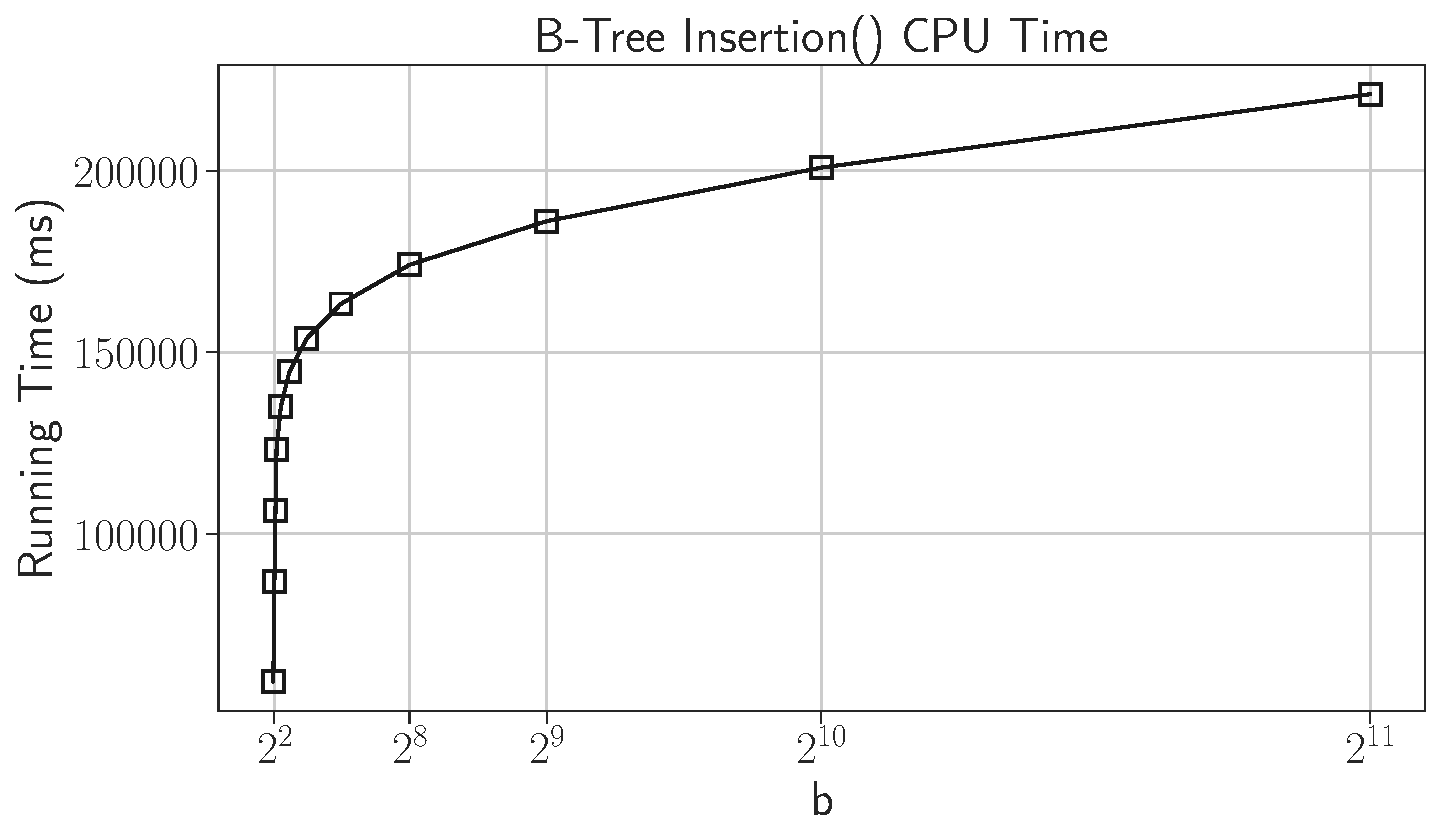
\includegraphics[width=\linewidth]{../notebook/plot/b-tree_insertion()_cpu_time.pdf}
		\label{fig:cpu_time}
	\end{minipage}\hfill
	\begin{minipage}{0.5\textwidth}
		\centering
		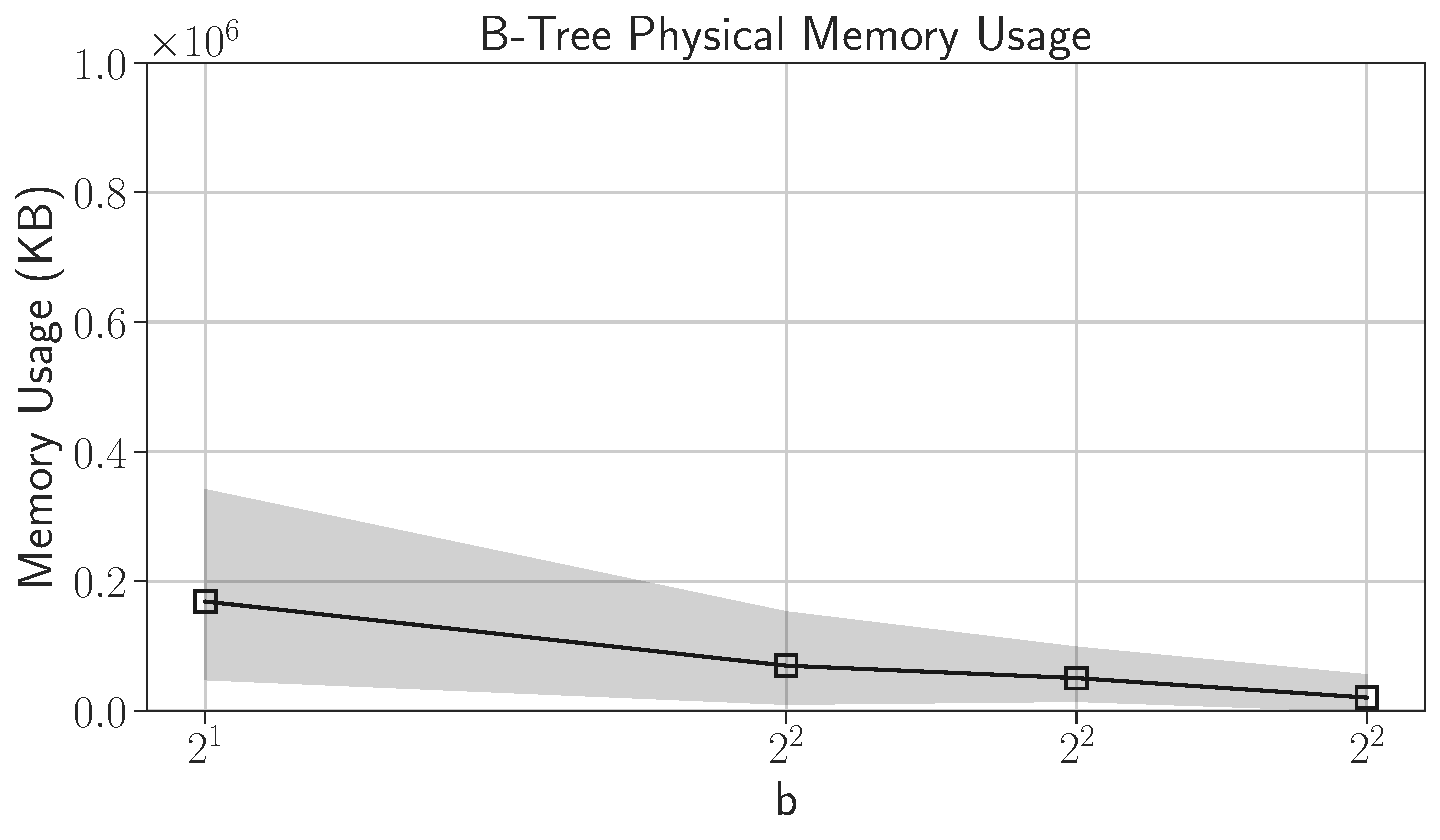
\includegraphics[width=\linewidth]{../notebook/plot/b-tree_physical_memory_usage.pdf}
		\label{fig:physical_memory}
	\end{minipage}\hfill
	\caption{CPU Time and Physcal Memory Usage for B-Tree insertion with varying $b$ values.}
\end{figure}

Notice that as the parameter of $b$ the B-Tree increases, the physical memory usage decreases. My theory is that increasing $b$ makes the tree shallower and more compact. Since a shallower tree reduces the number of pointers and improves spatial locality, nodes are more likely to fit within a cache line, leading to better memory efficiency?
\\\\
Anywhow... we want the b such that the it minimizes CPU time and memory used. They way I did it is to simply normalize CPU time and memory used and get closest b with to the smallest differnce. 

\begin{figure}[H]
	\centering
	\begin{minipage}{1\textwidth}
		\centering
		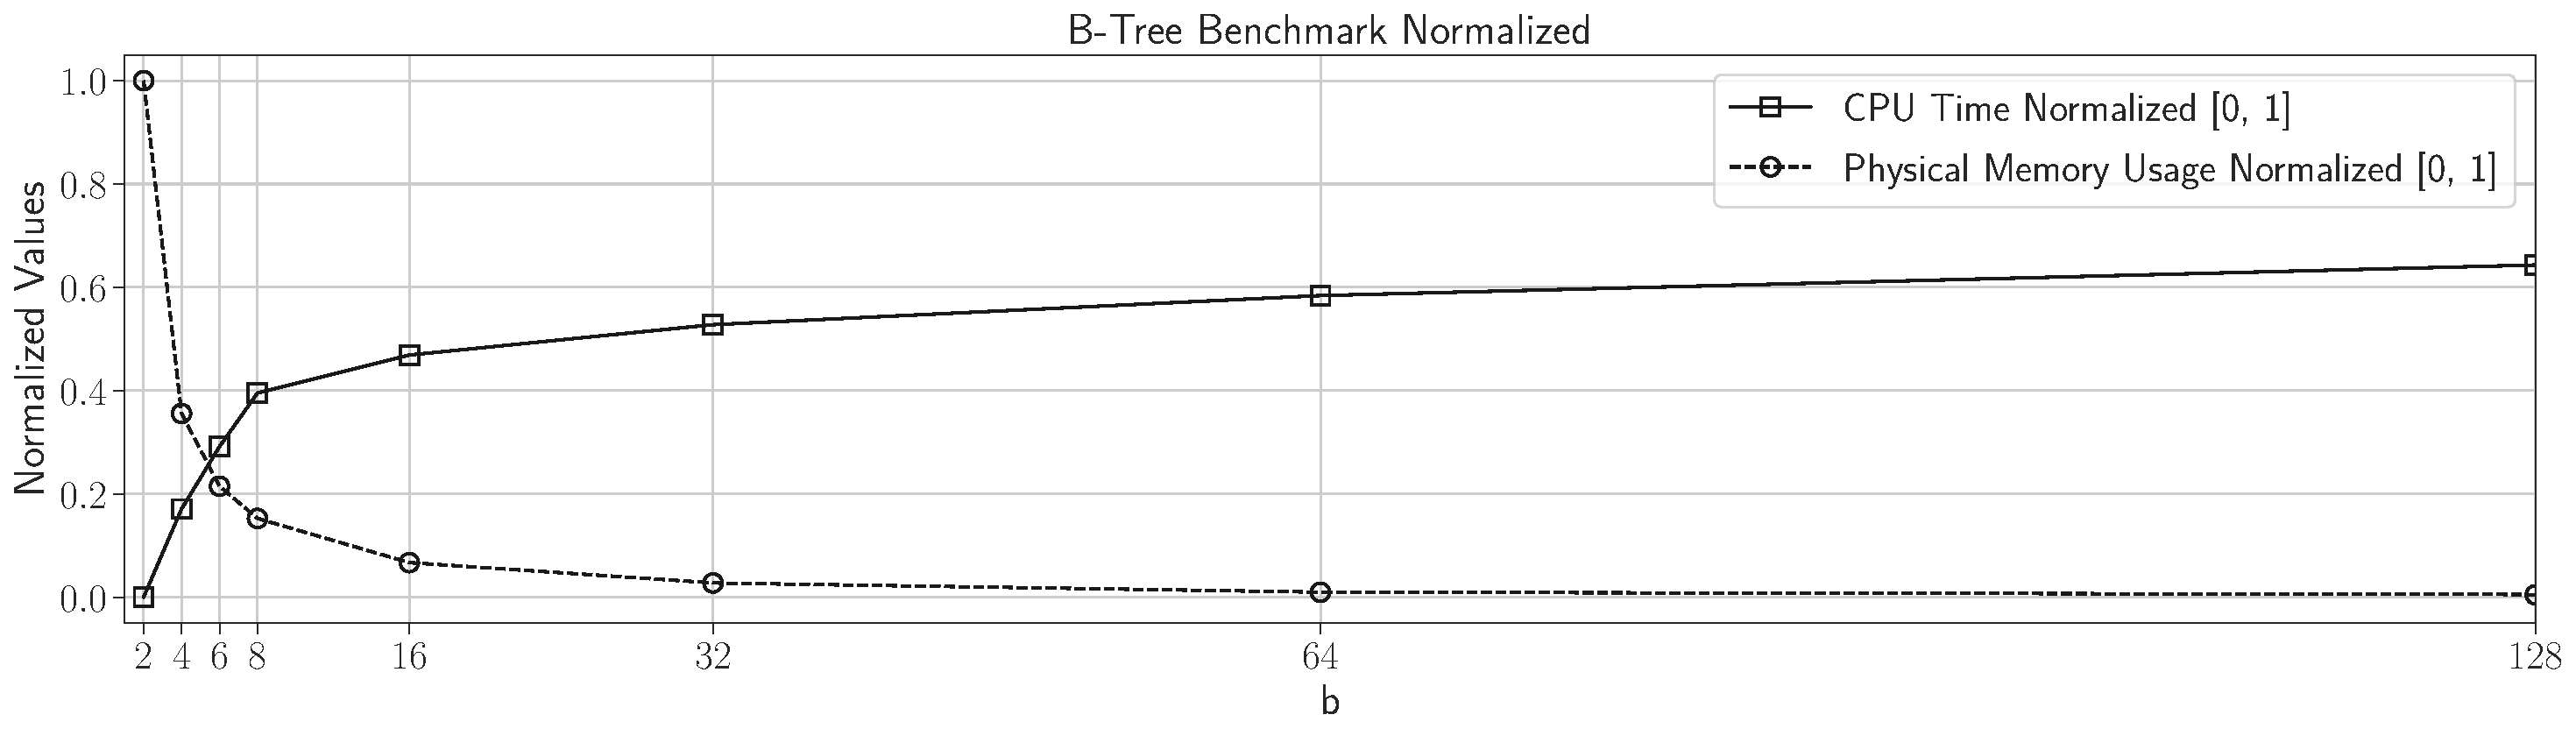
\includegraphics[width=\linewidth]{../notebook/plot/b-tree_benchmark_normalized.pdf}
		\label{fig:benchmark_normalized}
	\end{minipage}
	\caption{Normalized CPU Time and Physcal Memory Usage comparison for B-Tree insertion with varying $b$ values.}
\end{figure}

Setting $b = 6$ minimizes both performance overhead and memory usage the most. However, for applications that prioritize memory efficiency over execution time, a larger value, such as $b = 16$, may be more optimal, as the performance trade-off becomes less significant. This version clarifies that $b = 6$ minimizes both performance overhead and memory usage while improving the flow of the second sentence.

\subsubsection*{Comparing B-Tree and Builtin Ordered-Map Performance}


\begin{figure}[H]
	\centering
	\begin{minipage}{0.5\textwidth}
		\centering
		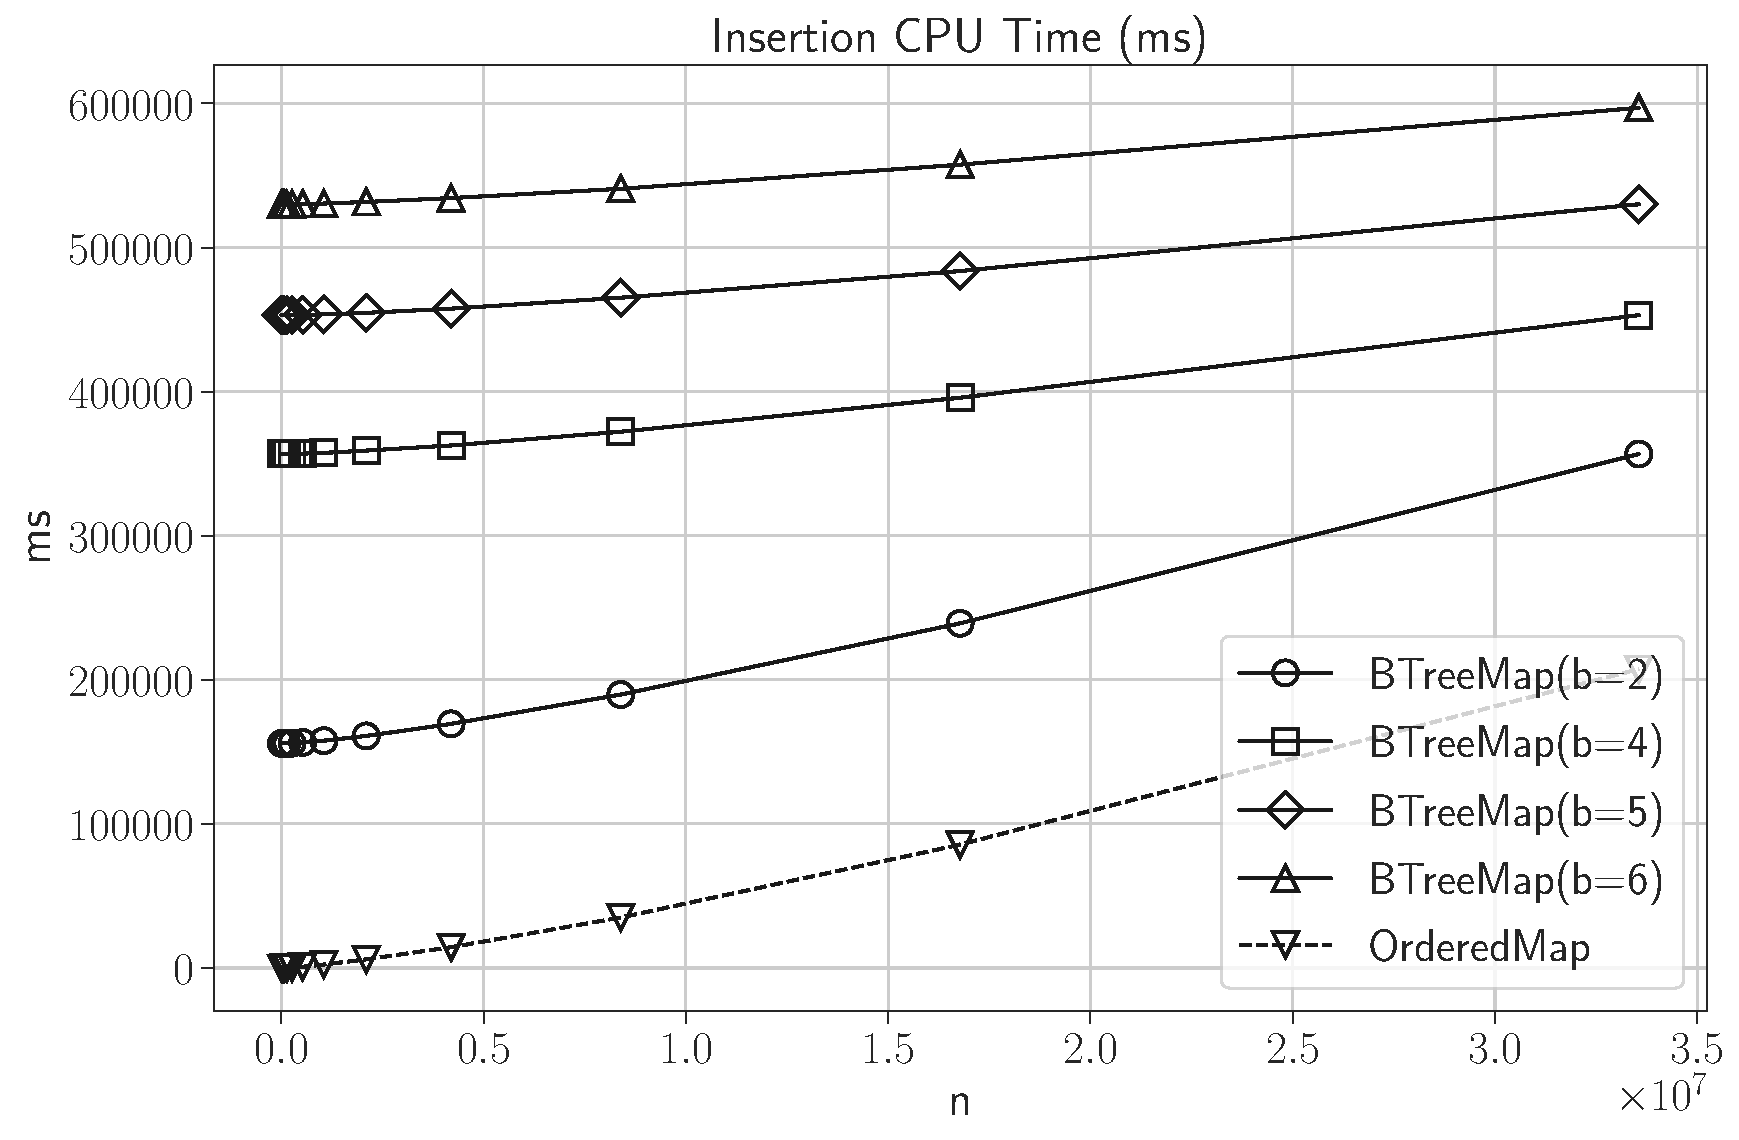
\includegraphics[width=1\linewidth]{../notebook/plot/insertion_cpu_time_(ms)}
	\end{minipage}\hfill
	\begin{minipage}{0.5\textwidth}
		\centering
		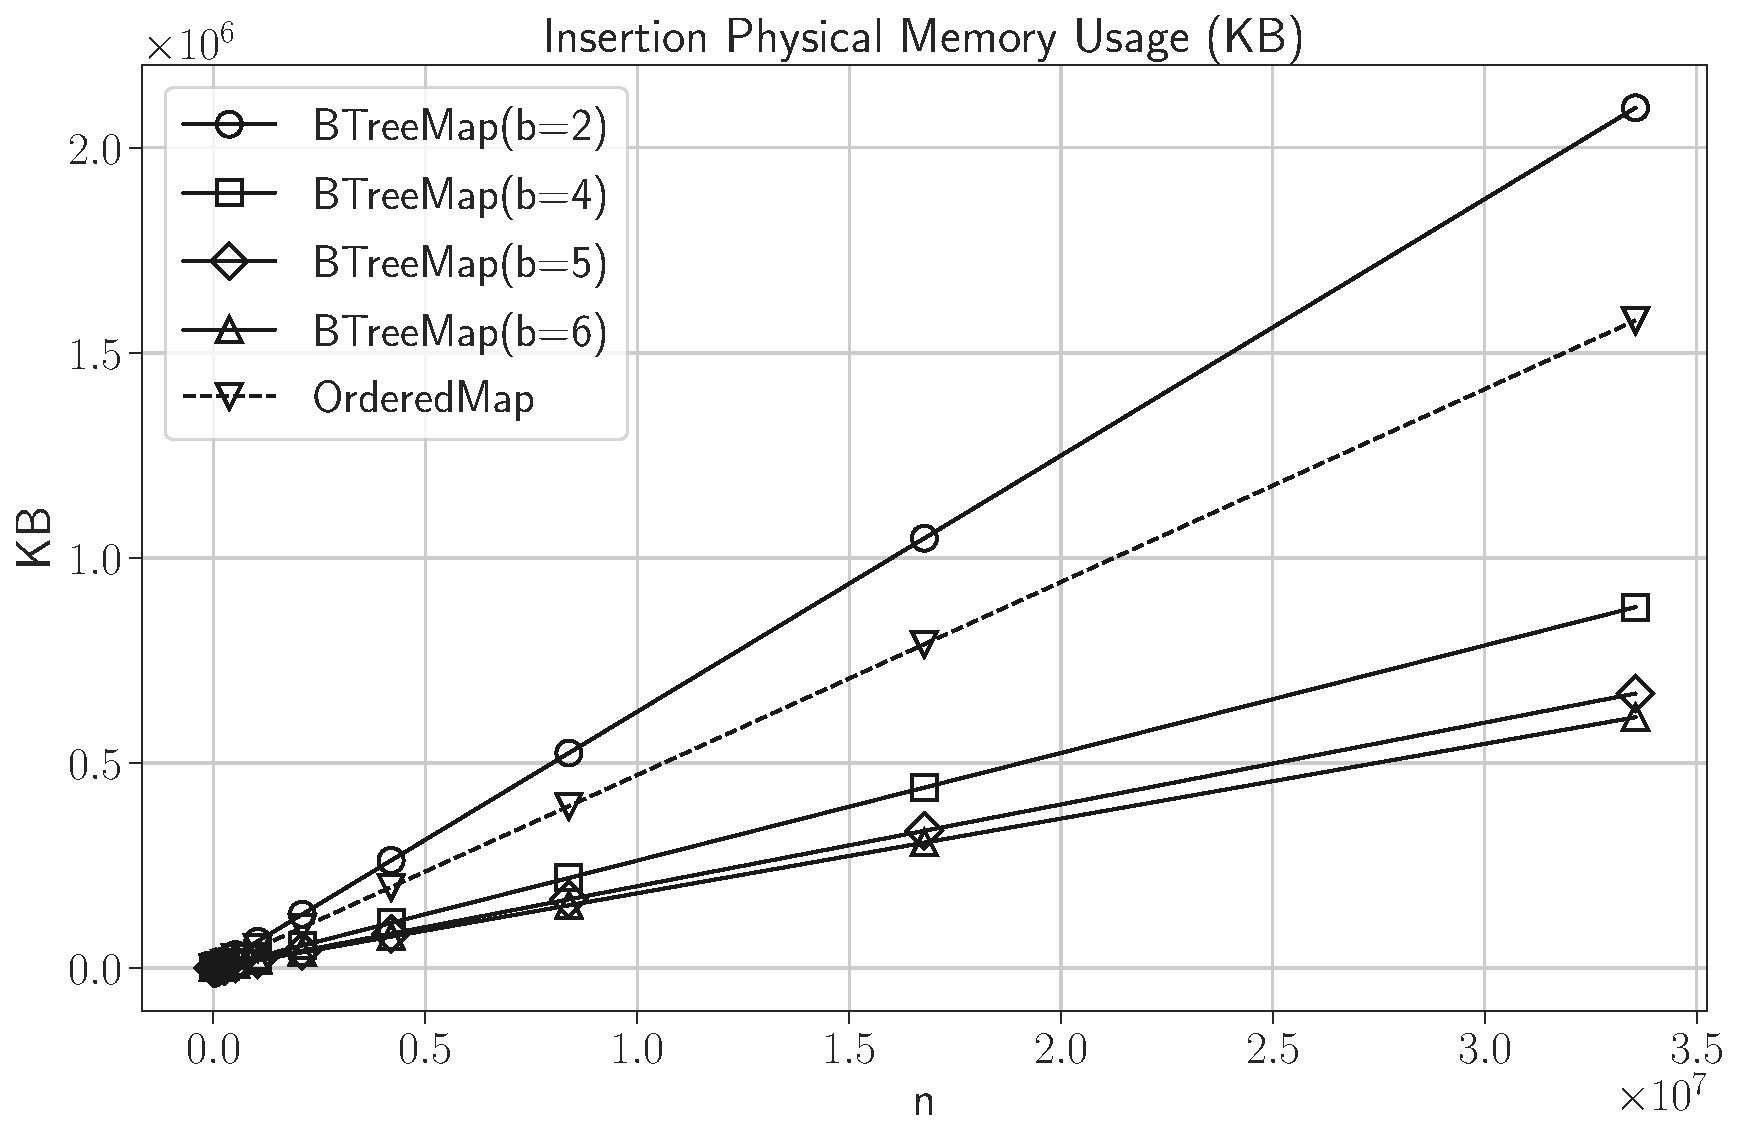
\includegraphics[width=1\linewidth]{../notebook/plot/insertion_physical_memory_usage_(kb)}
	\end{minipage}\hfill 
	\\
	\begin{minipage}{0.5\textwidth}
		\centering
		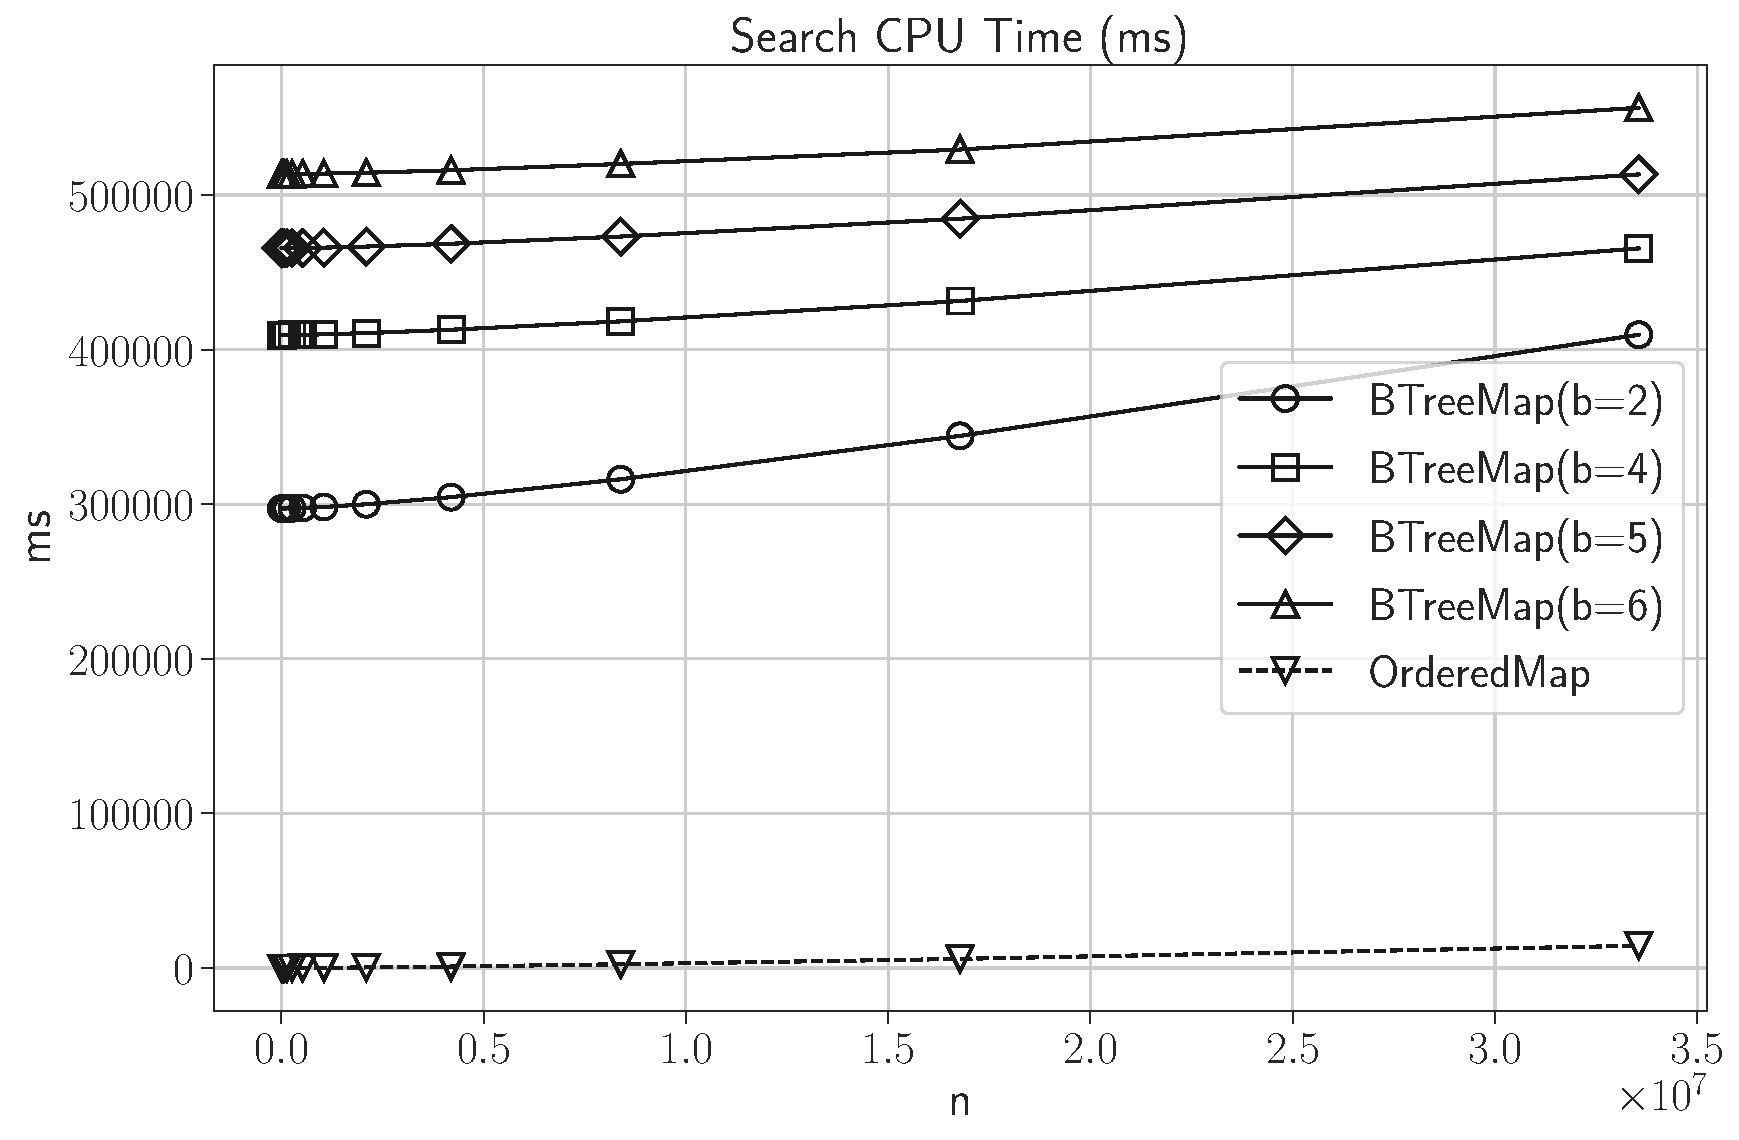
\includegraphics[width=1\linewidth]{../notebook/plot/search_cpu_time_(ms)}
	\end{minipage}\hfill

	\caption{CPU Time and Physcal Memory Usage of B-Tree and C++ Builtin Ordered Map. Inserted $2^{24}$ unique and random keys.}
	\label{fig:om_vs_bt}
\end{figure}




Figure~\ref{fig:om_vs_bt} illustrates that the running time for the C++ built-in Ordered Map outperforms the B-Tree in both insertion and search operations. However, it is important to note that for B-Trees with $b > 2$, memory efficiency improves, making them more memory-efficient than the built-in Ordered Map.


\noindent
\begin{minipage}{0.5\textwidth}
    \centering
	\resizebox{0.85\textwidth}{!}{%
		\begin{tabular}{rrr}
		\hline
		\multicolumn{3}{c}{\textbf{Ordered Map Insertion}} \\ \hline
		n             & CPU Time (ms)      & Memory Usage (KB)      \\ \hline
		8        & 0.00E+00 & 4       \\
		16       & 0.00E+00 & 0       \\
		32       & 0.00E+00 & 0       \\
		64       & 0.00E+00 & 0       \\
		128      & 0.00E+00 & 0       \\
		256      & 0.00E+00 & 4       \\
		512      & 0.00E+00 & 12      \\
		1024     & 0.00E+00 & 24      \\
		2048     & 0.00E+00 & 64      \\
		4096     & 0.00E+00 & 176     \\
		8192     & 0.00E+00 & 368     \\
		16384    & 3.13E+01 & 684     \\
		32768    & 1.56E+01 & 1584    \\
		65536    & 4.69E+01 & 3080    \\
		131072   & 1.41E+02 & 5936    \\
		262144   & 3.28E+02 & 11884   \\
		524288   & 8.91E+02 & 24628   \\
		1048576  & 2.42E+03 & 49260   \\
		2097152  & 6.02E+03 & 98572   \\
		4194304  & 1.44E+04 & 197348  \\
		8388608  & 3.51E+04 & 394748  \\
		16777216 & 8.57E+04 & 789744  \\
		33554432 & 2.08E+05 & 1579572 \\ \hline
		\end{tabular}
		}
\end{minipage}%
\hfill
\begin{minipage}{0.5\textwidth}
    \centering
	\resizebox{0.85\textwidth}{!}{%
		\begin{tabular}{rrr}
		\hline
		\multicolumn{3}{c}{\textbf{B-Tree $$b=6$$ Insertion}} \\ \hline
		n             & CPU Time (ms)      & Memory Usage (KB)      \\ \hline
		8        & 5.30E+05 & 4      \\
		16       & 5.30E+05 & 0      \\
		32       & 5.30E+05 & 0      \\
		64       & 5.30E+05 & 0      \\
		128      & 5.30E+05 & 4      \\
		256      & 5.30E+05 & 4      \\
		512      & 5.30E+05 & 8      \\
		1024     & 5.30E+05 & 16     \\
		2048     & 5.30E+05 & 32     \\
		4096     & 5.30E+05 & 68     \\
		8192     & 5.30E+05 & 124    \\
		16384    & 5.30E+05 & 308    \\
		32768    & 5.30E+05 & 576    \\
		65536    & 5.30E+05 & 1148   \\
		131072   & 5.30E+05 & 2216   \\
		262144   & 5.30E+05 & 4460   \\
		524288   & 5.30E+05 & 9356   \\
		1048576  & 5.31E+05 & 19092  \\
		2097152  & 5.32E+05 & 38316  \\
		4194304  & 5.34E+05 & 76508  \\
		8388608  & 5.41E+05 & 152888 \\
		16777216 & 5.58E+05 & 305684 \\
		33554432 & 5.97E+05 & 611656  \\ \hline
		\end{tabular}
	}
    % \captionof{table}{First Table}
\end{minipage}%

\vspace{14pt}

\noindent
\begin{minipage}{0.5\textwidth}
    \centering
	\resizebox{0.85\textwidth}{!}{%
		\begin{tabular}{rrr}
		\hline
		\multicolumn{3}{c}{\textbf{Ordered Map Search}} \\ \hline
		n             & CPU Time (ms)      & Memory Usage (KB)      \\ \hline
		8        & 3.07E-05 & 4       \\
		16       & 7.67E-05 & 0       \\
		32       & 1.71E-04 & 0       \\
		64       & 4.53E-04 & 0       \\
		128      & 9.63E-04 & 0       \\
		256      & 2.22E-03 & 4       \\
		512      & 4.46E-03 & 12      \\
		1024     & 2.93E-02 & 24      \\
		2048     & 9.42E-02 & 64      \\
		4096     & 2.68E-01 & 176     \\
		8192     & 6.28E-01 & 368     \\
		16384    & 1.38E+00 & 684     \\
		32768    & 3.29E+00 & 1584    \\
		65536    & 8.54E+00 & 3080    \\
		131072   & 2.34E+01 & 5936    \\
		262144   & 1.02E+02 & 11884   \\
		524288   & 2.66E+02 & 24628   \\
		1048576  & 8.13E+02 & 49260   \\
		2097152  & 2.06E+03 & 98572   \\
		4194304  & 5.06E+03 & 197348  \\
		8388608  & 1.43E+04 & 394748  \\
		16777216 & 3.06E+04 & 789744  \\
		33554432 & 7.36E+04 & 1579572 \\ \hline
		\end{tabular}
	}
\end{minipage}%
\hfill
\begin{minipage}{0.5\textwidth}
    \centering
	\resizebox{0.85\textwidth}{!}{%
		\begin{tabular}{rrr}
		\hline
		\multicolumn{3}{c}{\textbf{B-Tree $$b=6$$ Search}} \\ \hline
		n             & CPU Time (ms)      & Memory Usage (KB)      \\ \hline
		8        & 1.66E+06 & 4      \\
		16       & 1.66E+06 & 0      \\
		32       & 1.66E+06 & 0      \\
		64       & 1.66E+06 & 0      \\
		128      & 1.66E+06 & 4      \\
		256      & 1.66E+06 & 4      \\
		512      & 1.66E+06 & 8      \\
		1024     & 1.66E+06 & 16     \\
		2048     & 1.66E+06 & 32     \\
		4096     & 1.66E+06 & 68     \\
		8192     & 1.66E+06 & 124    \\
		16384    & 1.66E+06 & 308    \\
		32768    & 1.66E+06 & 576    \\
		65536    & 1.66E+06 & 1148   \\
		131072   & 1.66E+06 & 2216   \\
		262144   & 1.66E+06 & 4460   \\
		524288   & 1.66E+06 & 9356   \\
		1048576  & 1.66E+06 & 19092  \\
		2097152  & 1.66E+06 & 38316  \\
		4194304  & 1.67E+06 & 76508  \\
		8388608  & 1.68E+06 & 152888 \\
		16777216 & 1.72E+06 & 305684 \\
		33554432 & 1.81E+06 & 611656  \\ \hline
		\end{tabular}
	}
    % \captionof{table}{First Table}
\end{minipage}%

\vspace{14pt}


\begin{thebibliography}{9}
	\bibitem{google-bench} 
	Google Benchmark. 
	\textit{A microbenchmark support library}. 
	Available at: \url{https://github.com/google/benchmark}

	\bibitem{btree_github} 
	B-Tree Implementation on GitHub. 
	\textit{GitHub Repository}. 
	Available at: \url{https://github.com/frozenca/BTree}

	\bibitem{getprocessmemoryinfo} 
	GetProcessMemoryInfo function. 
	\textit{Microsoft Learn}. 
	Available at: \url{https://learn.microsoft.com/en-us/windows/win32/api/psapi/nf-psapi-getprocessmemoryinfo}

\end{thebibliography}

	
\end{document}